\documentclass{article} % This command is used to set the type of document you are working on such as an article, book, or presentation

\usepackage{geometry} % This package allows the editing of the page layout
\usepackage{amsmath}  % This package allows the use of a large range of mathematical formula, commands, and symbols
\usepackage{graphicx}  % This package allows the importing of images
\usepackage{enumerate} %This package allows the use of making lists
% Required packages
\usepackage[dvipsnames]{xcolor}
\usepackage{tikz}

\newcommand{\question}[2][]{\begin{flushleft}
        \textbf{Question #1}: \textit{#2}

\end{flushleft}}
\newcommand{\sol}{\textbf{Solution}:} %Use if you want a boldface solution line
\newcommand{\maketitletwo}[2][]{\begin{center}
        \Large{\textbf{Assignment 2}
            
            CS 2813 - Discrete Structures} % Name of course here
        \vspace{5pt}
        
        \normalsize{Lucas Ho  % Your name here
        
        September 20, 2023}        % Due date
        \vspace{15pt}
        
\end{center}}
\begin{document}
\maketitletwo[5]  % Optional argument is assignment number
    %Keep a blank space between maketitletwo and \question[1]
    
    \question[1]{Translate in two ways each of these statements into logical expressions using predicates, quantifiers, and logical connectives. first, let the domain consist of the students in your class and second, let it consist of all people.} 
    \begin{enumerate}[a)]
    \item {Everyone in your class has a cellular phone.}
    \item {Somebody in your class has seen a foreign movie.}
    \item {There is a person in your class who cannot swim.}
    \item {All students in your class can solve quadratic equations.}
    \item {Some student in your class does not want to be rich.}
    \end{enumerate}
    Let x be a person and C(x) is a propositional function for "x is in your class."
    \begin{enumerate}[a)]
      \item {Let F(x) be "x has a cellular phone." Then $\exists$xF(x) for the first domain and $\forall$x(C(x) $\rightarrow$ F(x)) for the second domain.}
      \item {Let G(x) be "x has seen a foreign movie." Then $\exists$xG(x) for the first domain and $\exists$x(C(x) $\land$ G(x)) for the second domain.}
      \item {Let H(x) be "x can swim." Then $\exists$x$\neg$H(x) for the first domain and $\exists$x(C(x) $\land$ $\neg$H(x)) for the second domain.}
      \item {Let J(x) be "x can solve quadratic equations. Then $\forall$xJ(x) for the first domain and $\forall$x(C(x) $\rightarrow$ J(x)) for the second domain.}
      \item {Let K(x) be "x wants to be rich." Then $\exists$x$\neg$K(x) for the first domain and $\exists$x(C(x) $\land$ $\neg$K(x)) for the second domain.}
    \end{enumerate}

    \question[2]{Suppose the domain of the propositional function P(x, y) consists of pairs x and y, where x is 1, 2, or 3 and y is 1, 2, or 3. Using these values, write out these propositions using disjunctions and conjunctions.}
    \begin{enumerate}[a)]
      \item {$\exists$xP(x, 3)}
      
      P(1,3) $\lor$ P(2,3) $\lor$ P(3,3)
      
      \item {$\forall$yP(1, y)}
      
      P(1,1) $\land$ P(1,2) $\land$ P(1,3)

      \item {$\exists$y$\neg$P(2, y)}
      
      $\neg$P(2,1) $\lor$ $\neg$P(2,2) $\lor$ $\neg$P(2,3)

      \item {$\forall$x$\neg$P(x, 2)}
      
      $\neg$P(1,2) $\land$ $\neg$P(2,2) $\land$ $\neg$P(3,2)
    \end{enumerate}

  \question[3]{Determine the truth value of each of these statements if the domain of each
  variable consists of all real numbers.}
  \begin{enumerate}[a)]
    \item {$\forall$x$\exists$y(x$\textsuperscript{2}$ = y)}
    
    T The square of a real number is a real number.

    \item {$\forall$x$\exists$y(x = y$\textsuperscript{2}$)}
    
    F There are no real numbers that can be squared to equal a negative number.
    \item {$\exists$x$\forall$y(xy = 0)}
    
    T x can be equal to zero to for all values of y to make this statement true.
    \item {$\exists$x$\exists$y(x + y $\neq$ y + x)}
    
    F By the Associative Law of arithmetic, this statement is false.
    \item {$\exists$x$\exists$y(x + 2y = 2 $\land$ 2x + 4y = 5)} 
    
    F Both of these statements represent the equation of a line and these two line equations are parallel to each other.
    
  \end{enumerate}

  \question[4]{Show that if A, B, and C are sets, then $\mid$A $\cup$ B $\cup$ C$\mid$ = $\mid$A$\mid$ + $\mid$B$\mid$ + $\mid$C$\mid$ - $\mid$A $\cap$ B$\mid$ - $\mid$A $\cap$ C$\mid$ - $\mid$B $\cap$ C$\mid$ + $\mid$A $\cap$ B $\cap$ C$\mid$.}

  $\mid$A$\mid$ = x,
  $\mid$B$\mid$ = y,
  $\mid$C$\mid$ = z

  First include all of the cardinality of the sets

  x + y + z

  Then remove the redundant intersections

  x $\cap$ y + x $\cap$ z + y $\cap$ z

  Then account for intersection of all three sets that was removed when accounting for redundant intersections

  x $\cap$ y $\cap$ z

  Combining all these together forms

  x + y + z - x $\cap$ y - x $\cap$ z - y $\cap$ z + x $\cap$ y $\cap$ z

  Substituting the values back in and we get the same results in the beginning

  $\mid$A$\mid$ + $\mid$B$\mid$ + $\mid$C$\mid$ - $\mid$A $\cap$ B$\mid$ - $\mid$A $\cap$ C$\mid$ - $\mid$B $\cap$ C$\mid$ + $\mid$A $\cap$ B $\cap$ C$\mid$


  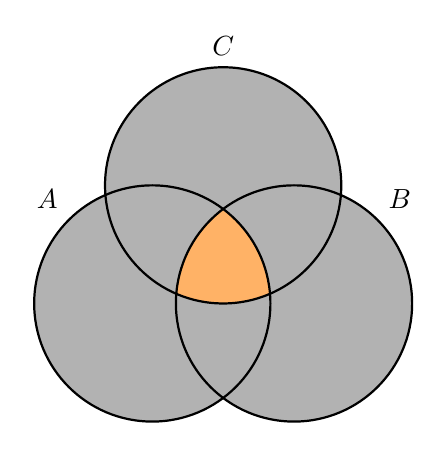
\begin{tikzpicture}[thick,
    set/.style = {circle,
      minimum size = 3cm,
      fill=black!30}]
  
  % Set A
  \node[set,label={135:$A$}] (A) at (0,0) {};
  
  % Set B
  \node[set,label={45:$B$}] (B) at (1.8,0) {};
  
  % Set C
  \node[set,label=$C$] (C) at (0.9,1.5) {};
  
  % Intersection
  \begin{scope}
    \clip (0,0) circle(1.5cm);
    \clip (1.8,0) circle(1.5cm);
    \clip (0.9,1.5) circle(1.5cm);
    \fill[orange!60](0,0) circle(1.5cm);
  \end{scope}
  
  % Circles outline
  \draw (0,0) circle(1.5cm);
  \draw (1.8,0) circle(1.5cm);
  \draw (0.9,1.5) circle(1.5cm);
  
  \end{tikzpicture}

  \question[5]{Suppose that the universal set is U = 1, 2, 3, 4, 5, 6, 7, 8, 9, 10. Express each of
  these sets with bit strings where the ith bit in the string is 1 if i is in the set and 0 otherwise.}

  \begin{enumerate}[a)]
    \item {3, 4, 5}
    
    0011100000
    \item {1, 3, 6, 10}
    
    1010010001
    \item {2, 3, 4, 7, 8 , 9}
    
    01110001110
    
  \end{enumerate}

  \question[6]{Given the following Algorithm 1: }

  \begin{enumerate}[a)]
    \item{Can we check if x == a$\textsubscript{j}$ instead of if x == a$\textsubscript{i}$? Why?}
    
    Yes, if we check for a$\textsubscript{j}$ instead of a$\textsubscript{i}$ then the loop will end when a$\textsubscript{j}$ == a$\textsubscript{i}$ already.

    \item {Can we check if x == a$\textsubscript{m}$ instead of if x == a$\textsubscript{i}$? Why?}
    
    No, if check for a$\textsubscript{m}$ instead of a$\textsubscript{i}$ then the loop will end prematurely before getting the correct location.
    
  \end{enumerate}

  \question[7]{For n pairs of socks (2n total socks), how many iterations (pick up a sock, pick up another and check if they match to pair them) are in the best- and worst-case scenarios?}

  Best-case scenerio is one iterations to find a matching pair. Worst-case scenerio is 2n - 1 iterations.

  \question[8]{Show that}

  $\forall$xP(x) $\lor$ $\forall$xQ(x) and

  $\forall$x$\forall$y(P(x) $\lor$ Q(x)),
  
  where all quantifiers have the same nonempty domain, are logically equivalent. (The new variable y is used
  to combine the quantifications correctly).

  if $\forall$xP(x) $\lor$ $\forall$xQ(x) = $\forall$x$\forall$x(P(x) $\lor$ Q(x))

  Then substituting y = x, we get

  $\forall$x$\forall$y(P(x) $\lor$ Q(x))

\end{document}